% Chapter 1

\chapter{Automatic Metadata Extraction} % Main chapter title

\label{Chapter3} % For referencing the chapter elsewhere, use \ref{Chapter1} 

\lhead{Chapter 3. \emph{Automatic Metadata Extraction}} % This is for the header on each page - perhaps a shortened title

%----------------------------------------------------------------------------------------

\emph{In this chapter we define the problem of automatic metadata extraction and discuss the methods by which the problem may be solved. Moreover, we introduce GROBID, the metadata extraction tool around which our work is based, and describe the cascade of CRF models it uses to solve the problem. Notably, we provide a comparison between GROBID and the existing solution for metadata extraction at CERN, `REFEXTRACT'.}

\section{Metadata Extraction}

Automatic metadata extraction (AME) has been referred to as `one of the hardest problems in document engineering'. In our work we are concerned with extraction for scientific articles that are usually (though not necessarily) in the form of a PDF document, as these predominate in the INSPIRE-HEP digital library. Nevertheless, the same techniques will be effective for books, theses, or may even have novel applications\footnote{Such as for segmenting cooking recipes, as reported in The New York Times (http://open.blogs.nytimes.com/2015/04/09/extracting-structured-data-from-recipes-using-conditional-random-fields/?\_r=0).}. At CERN, the problem has been partially solved, albeit in a rudimentary way, and also entails a lot of manual curation to complete the work. See Section \ref{subsec:refextract} for a comparison between this existing solution and GROBID, the leading tool for metadata extraction.

\emph{Metadata} refers to various information explicitly or implicitly contained in a scientific article. Perhaps the most important metadata for an article is that contained in the header, that is, the text at the front of a document, typically containing the title of the article as well as the names, affilations and often the contact details of the authors, concluding finally with the article abstract. As a general rule, this is tantamount to the text of the document falling before the first section of the body (usually called 'Introduction'), though as we find in Chapter \ref{Chapter4}, sometimes significant amounts of front matter is held in unexpected places. Other important types of metadata may be the references of the article, typically classified into fields such as publication title, authors, data of publication, and so on. Another potential metadata type is that of the document structure, its chapters and sections. All of these types are modelled by GROBID.

\emph{Extraction} could refer to either of two distinct concepts. First, it may be the parsing of a PDF document and extraction of plaintext and images. This in itself is a complex problem, and may involve machine learning techniques for OCR analysis, depending on the rendering of the document. Or, it may be the  \emph{classification} of document content into predefined categories. It is on the second idea that we are focused within this work. Indeed, GROBID addresses both of these points, but the first is merely a precondition for the analysis it is primarily concerned with, and it houses a third-party PDF to XML conversion tool, \emph{pdftoxml}, developed at Xerox Research Centre Europe (XRCE), to handle this (\cite{dejean2006system}).

To appreciate the difficulty of automating such a task, consider Figure \ref{fig:headers}, contrasting the header sections of two articles from our dataset. Though the same sorts of information are present in both headers--title, author names, affilations, and document abstract--the arrangement and presentation of these fields are different, for example the sizing and placement of the document title, the juxtapositioning of authors (which are in variable in number) and author details, and labelling of the abstract block. Furthermore, the second header is more complete, in that it contains information not present in the other, for example copyright and publication details. The contents of a document header do not follow a predictable sequencing, making the problem hard, but are not entirely random, a condition that would render the problem impossible to solve. There is structure to a document, but it is likely infeasible to model deterministically. Therefore, we must look to probabilistic approaches, and accept that these will be error-prone.

\begin{figure}[!ht]
\subfloat[Header of article on CRFs.\label{subfig-1:dummy}]{%
  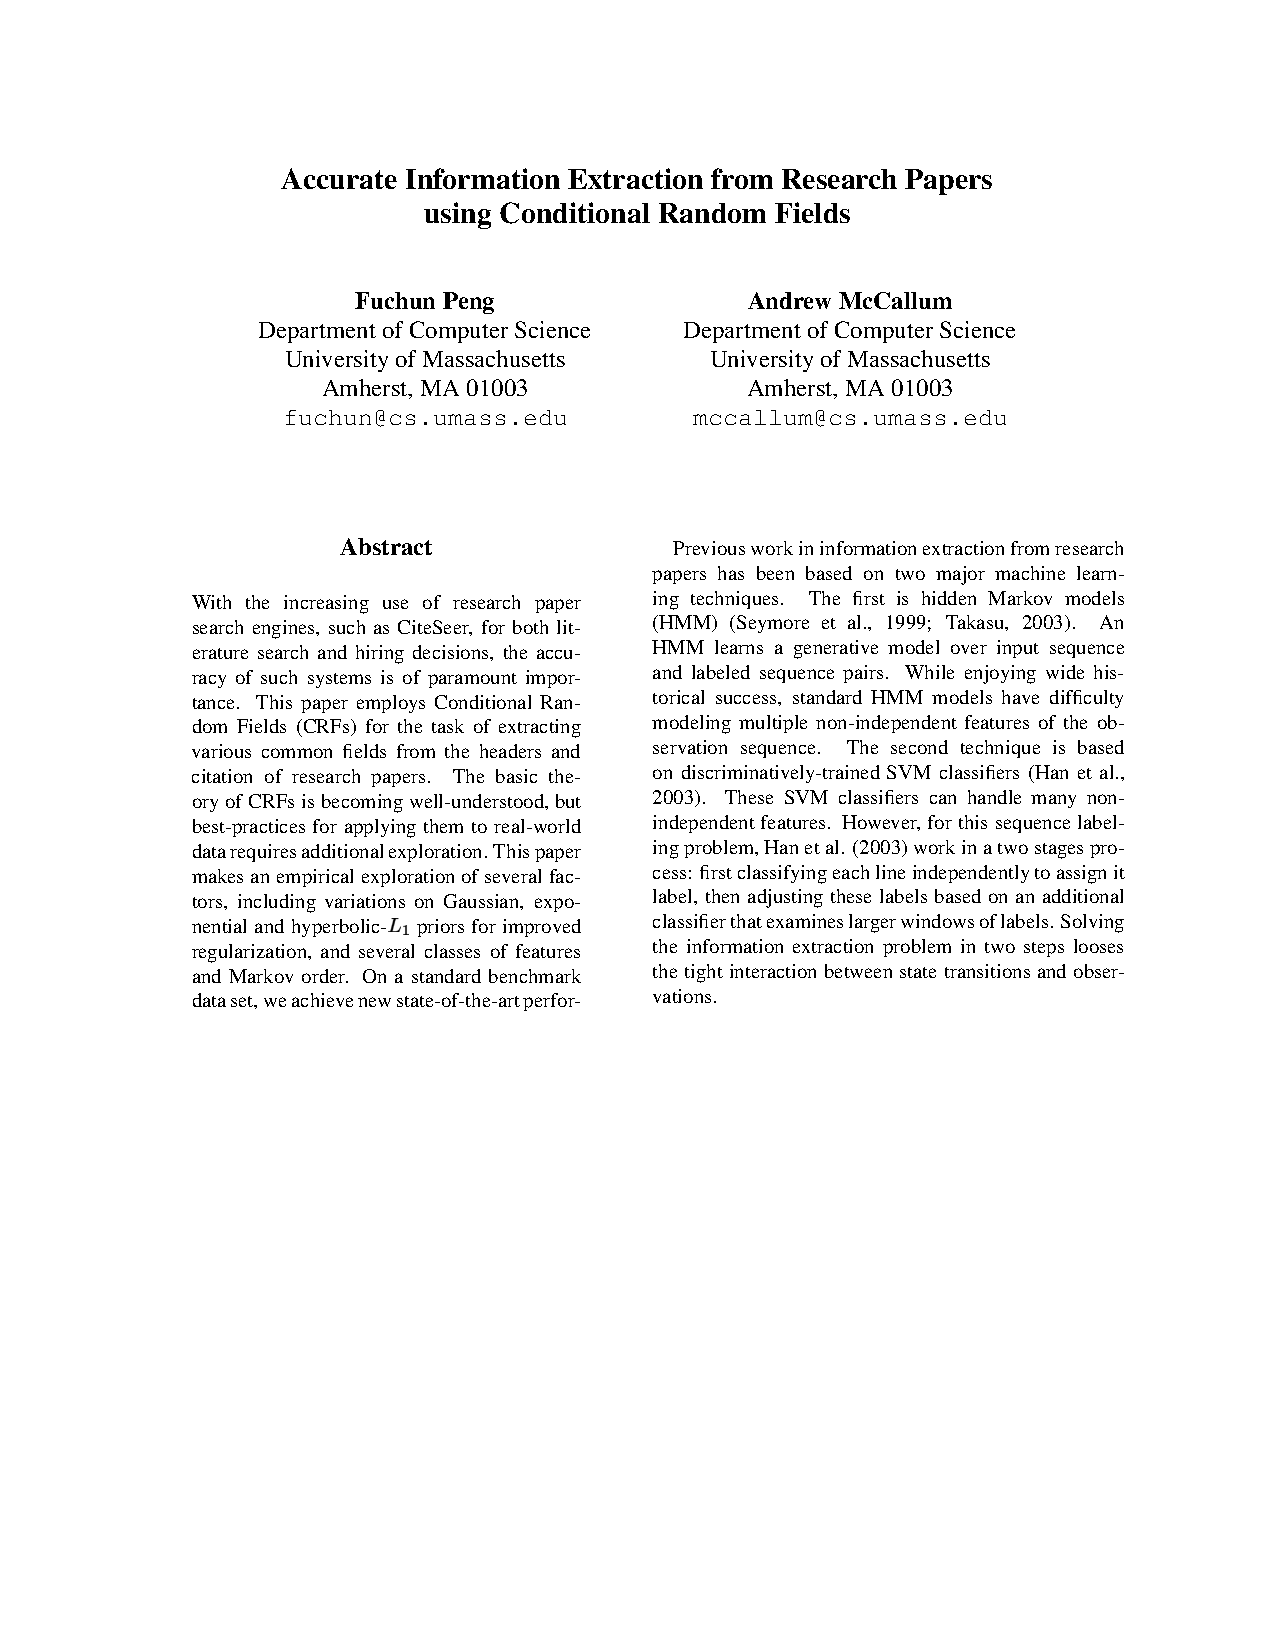
\includegraphics[width=0.45\textwidth]{Figures/header1.pdf}
}
\hfill
\subfloat[Header of HEP paper.\label{subfig-2:dummy}]{%
  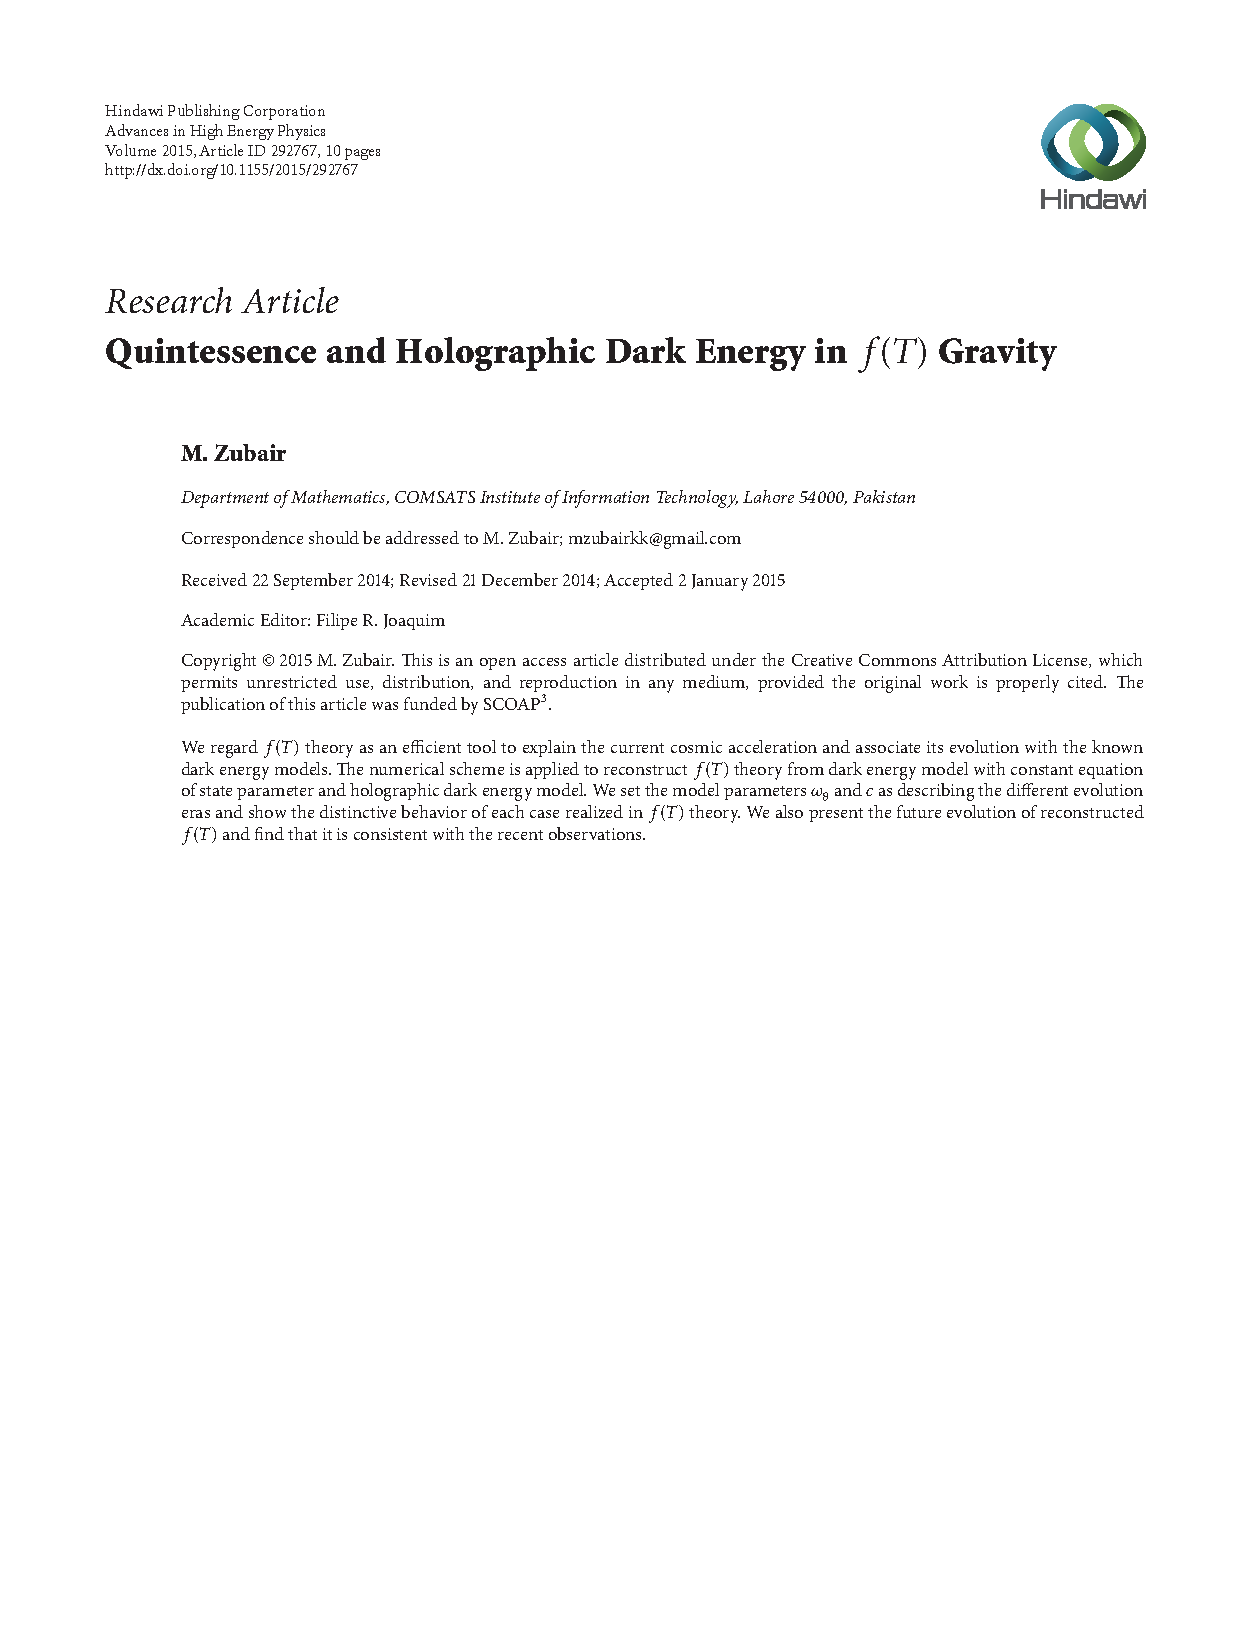
\includegraphics[width=0.45\textwidth]{Figures/header2.pdf}
}
\caption{Two differing header sections of articles from our dataset.}
\label{fig:headers}
\end{figure}

\section{Solution Methods}

Three main approaches have been considered for AME. They are:

\begin{enumerate}
\item template-based;
\item knowledge base, and;
\item machine learning approaches.
\end{enumerate}

There is evidence to suggest the best approach is a combination of the three.

Mention here the different solution types. Also mention the paper comparison used to select GROBID.

\section{GROBID}
\label{sec:grobid}
GROBID (https://github.com/kermitt2/grobid) is a Java-based tool for automatic metadata extraction 

\begin{figure}[!ht]
\center
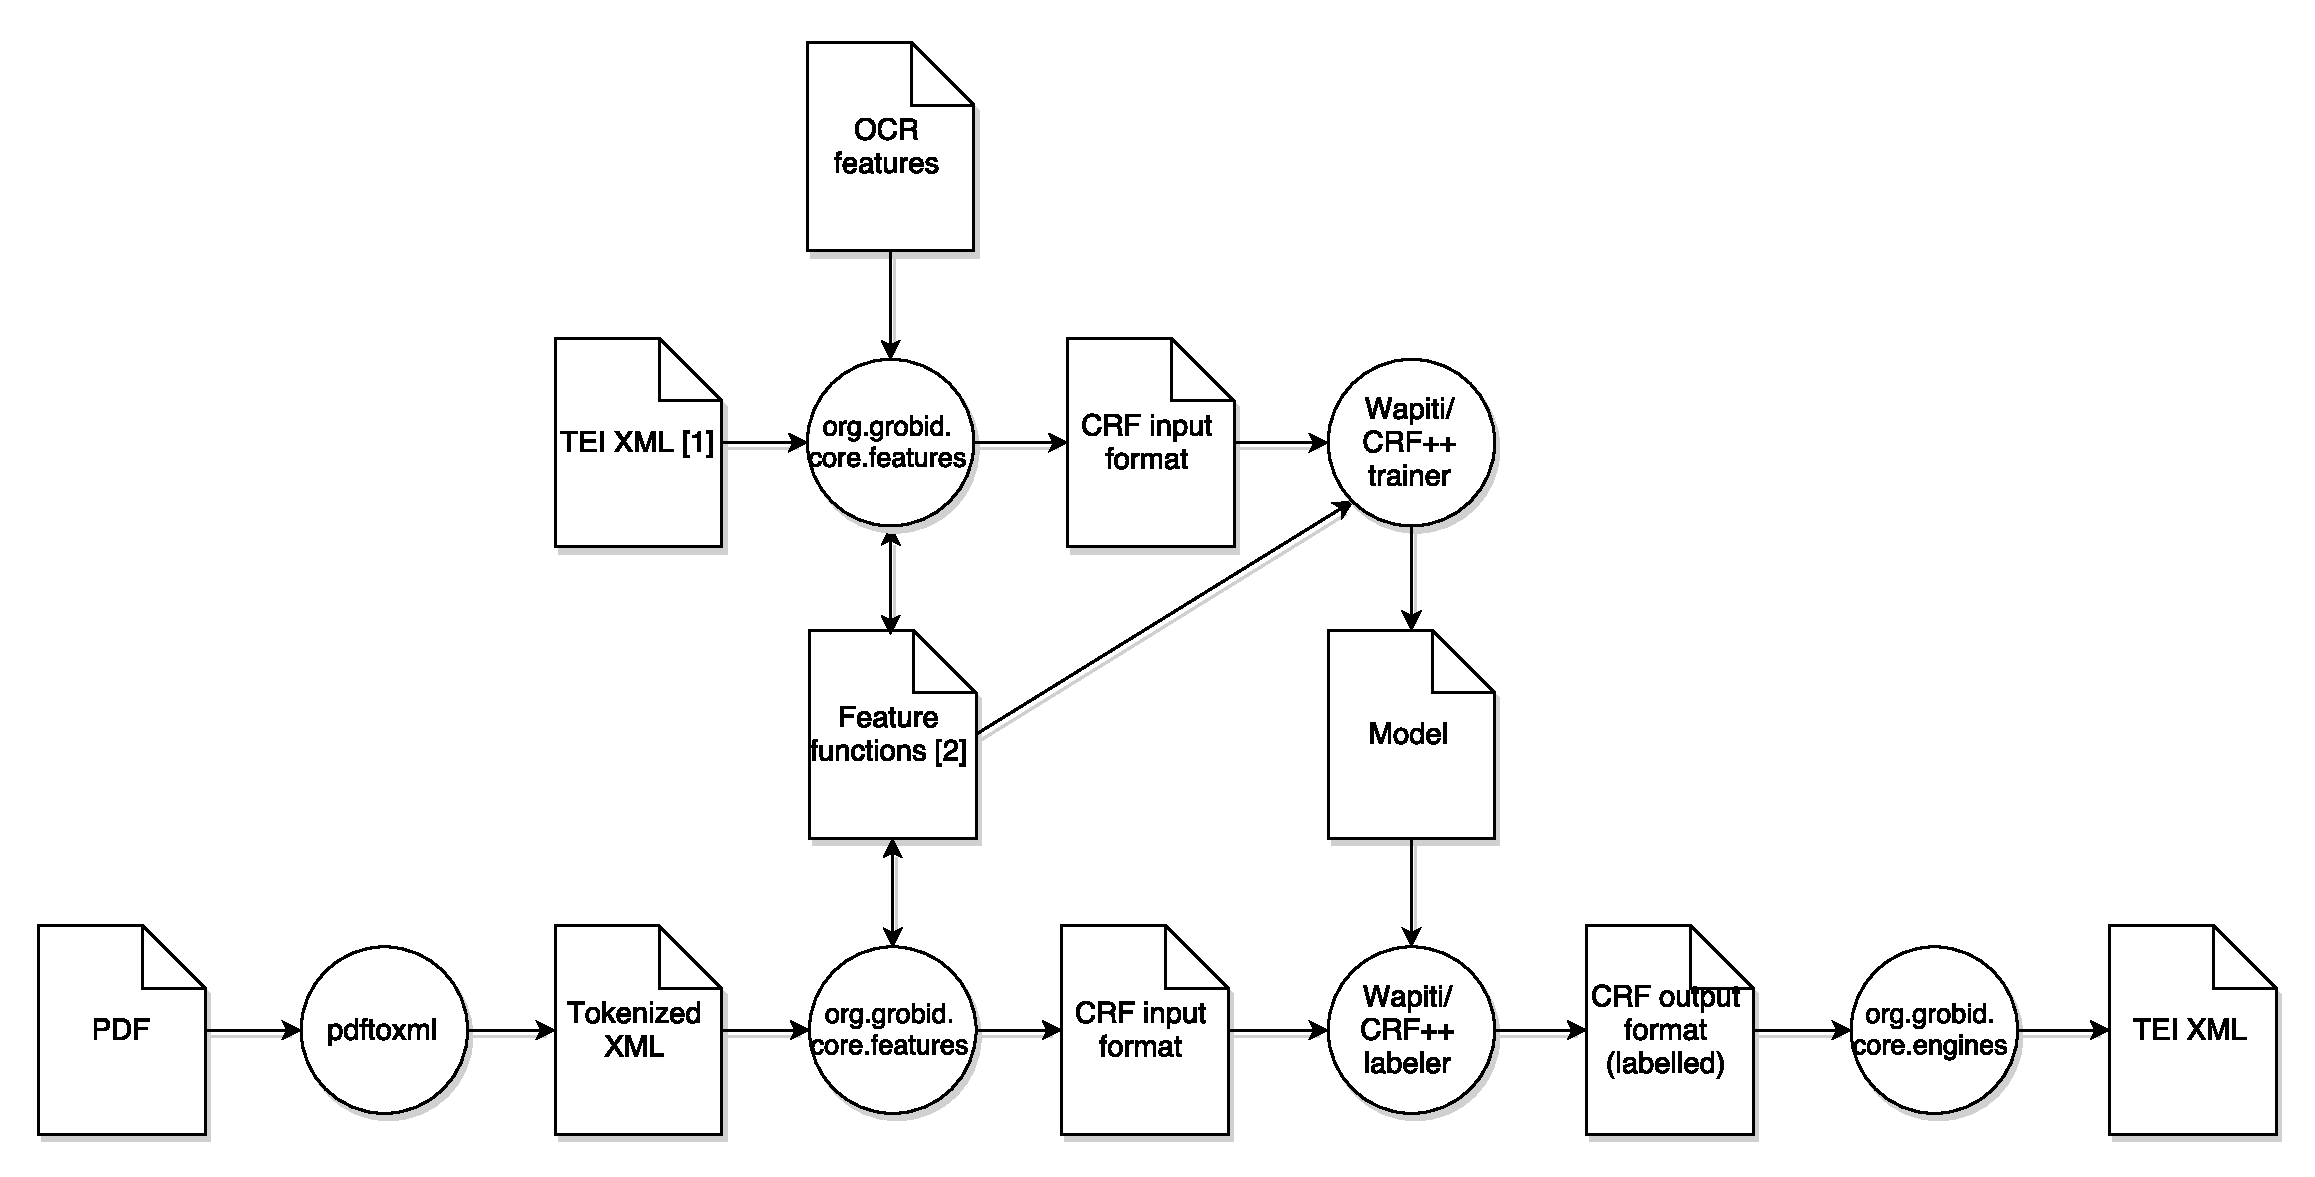
\includegraphics[width=\textwidth]{Figures/grobid.pdf}
\caption{An illustration of the interactions between Grobid and Wapiti for the two main functions of training and tagging.}
\label{fig:grobid}
\end{figure}

\begin{figure}[!ht]
\center
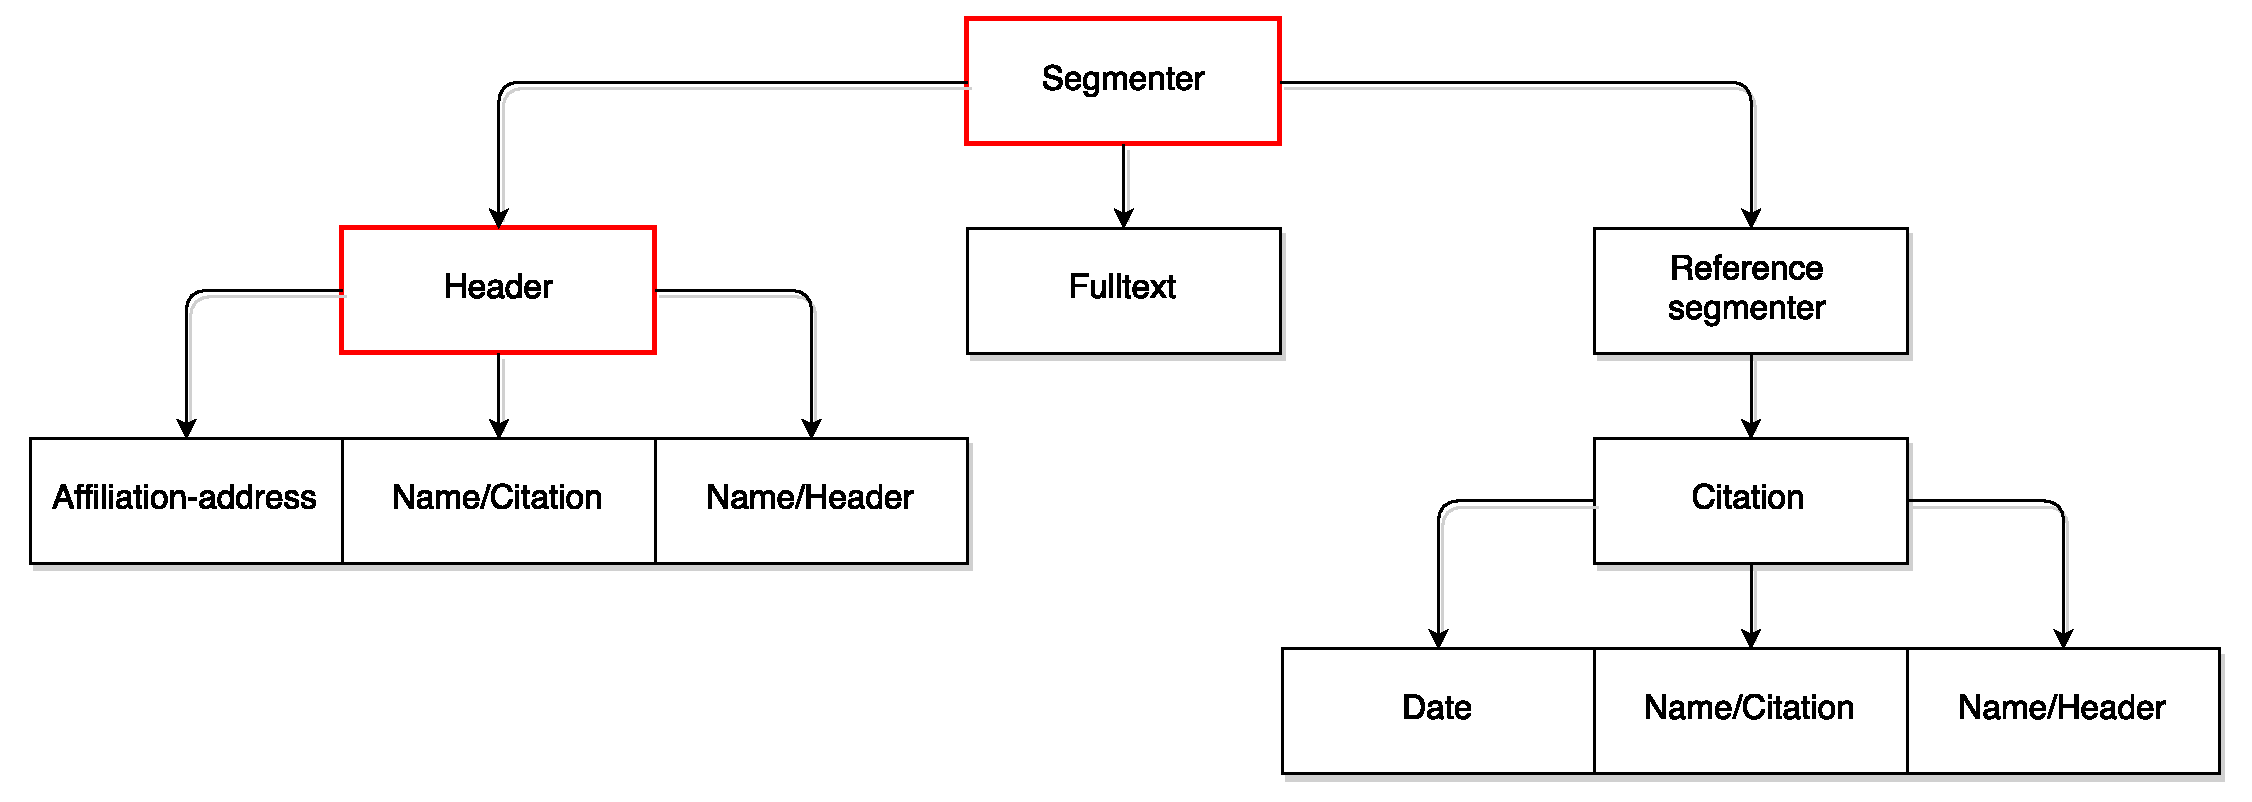
\includegraphics[width=\textwidth]{Figures/cascade.pdf}
\caption{The models of Grobid are organised into a cascade, where each part of a document is classified in increasingly greater detail.}
\label{fig:cascade}
\end{figure}

\subsection{Text Encoding Initiative}

One of GROBID's features is to transform Wapiti outputs into a standard output conforming to the Text Encoding Initiative (TEI)stanard, therefore we briefly describe it here. TEI is a text encoding standard maintained by the TEI constortium. It specifies an XML representation of a document contents from the front matter, to the document body, to the document rear. It gives structure and semantic meaning to document components, with little restriction to the level of detail desired. It is therefore apt as a file format for annotating a document's metadata. GROBID uses TEI to format its outputs, as well as its training data. In Figure \ref{fig:teicitation} we show a sample of a TEI document used to represent a date. The structured XML format gives information about the class of each of the tokens in a sequence.

\begin{figure}
\lstset{language=XML}
\begin{lstlisting}
<bibl>
    <author>V. Gundelach and D. Eisenburger</author>, &quot; 
    <title level="a">Principle of a direction sensitive borehole antenna with advanced technology and data examples</title>, &quot; in 	
    <title level="m">Proceedings of the 4th International Workshop on Advanced Ground Penetrating Radar (IWAGPR &apos;07)</title>, pp. 
    <biblScope type="pp">28-31</biblScope>, 
    <date>June 2007</date>.
</bibl>
\end{lstlisting}
\label{fig:teicitation}
\caption{Sample tagged citation for Grobid training input.}
\end{figure}

\subsection{Comparison with REFEXTRACT}
\label{subsec:refextract}
\begin{table}[h]
\begin{center}
\begin{tabular}{|c|cccc|}
\hline
label		&accuracy	&precision	&recall		&f1 \\
\hline
<label>		&99.96		&100		&99.2		&99.6\\
<reference>		&99.96		&99.96		&100		&99.98\\
\hline
(micro average) & 99.96		&99.96		&99.96		&99.96	\\
(macro average) &	99.96 & 99.98	& 99.6 & 99.79	\\
\hline
\end{tabular}
\caption[Table caption text]{Evaluation results for reference segmentation}
\end{center}
\end{table}

\begin{table}[h]
\begin{center}
\begin{tabular}{|c|cccc|cccc|}
\hline
engine &  \multicolumn{4}{c}{GROBID} & \multicolumn{4}{c}{REFEXTRACT}\\
\hline
label & accuracy & precision & recall & f1 & acc. & prec. & rec. & f1\\
\hline
<author>	&	99.85	&	99.68	&	99.75	&	99.72 	& 98.33	&	100	&	92.22	&	95.95	\\
<title>	&	99.59	&	98.87	&	99.25	&	99.06 	& 94.89	&	100	&	71.75	&	83.55	\\
<journal>	&	98.84	&	88.87	&	93.98	&	91.35 	& 97.12	&	100	&	46.78	&	63.74	\\
<volume>&	99.95	&	99.07	&	98.15	&	98.6 		& 98.36	&	0	&	0		&	0	\\
<issue>	&	99.93	&	100		&	94.63	&	97.24	 & 98.87	&	0	&	0		&	0	\\
<pages>	&	99.75	&	93.51	&	99.45	&	96.39 	& 97.26	&	0	&	0		&	0	\\
<date>	&	98.39	&	57.39	&	98.31	&	72.47 	& 98.88	&	100	&	37.55	&	54.6	\\
<pubnum>&	98.71	&	100		&	12.96	&	22.95 	& 98.77	&	0	&	0		&	0	\\
<note>	&	99.4	 	&	43.75	&	35		&	38.89 	& 99.55	&	0	&	0		&	0	\\
<publisher>&	99.81	&	63.46	&	94.29	&	75.86 	& 99.73	&	0	&	0		&	0	\\
<location>&	99.81	&	86.32	&	91.11	&	88.65 	& 99.32	&	0	&	0		&	0	\\
<institution>&	99.78	&	25		&	25		&	25 		& 99.88	&	0	&	0		&	0	\\
<booktitle>&	98.7		&	55.56	&	41.67	&	47.62 	& 98.82	&	0	&	0		&	0	\\
<web>	&	99.64	&	51.85	&	100		&	68.29 	& 99.68	&	0	&	0		&	0	\\
<editor>	&	99.93	&	100		&46.67		&	63.64 	& 99.89	&	0	&	0		&	0	\\
<tech>	&	99.95	&	83.33	&	50		&	62.5 		& 99.92	&	0	&	0		&	0	\\
\hline
(micro average) & 99.5	&	93.63	&	94.77 	&	94.19 & 98.7	&	100	&	63.47 	&	77.65	\\
(macro average) & 99.5	&	77.92	&	73.76	&	71.76 & 98.7	&	25	&	15.52	&	18.62	\\
\hline
\end{tabular}
\caption[Table caption text]{Evaluation results for citations}
\end{center}
\end{table}
